\documentclass[10pt]{extarticle}
\usepackage[utf8]{inputenc}
\usepackage{graphicx}
\usepackage{caption}
\usepackage{amsmath}
\usepackage{amssymb}
\usepackage{amsfonts}
\usepackage{listings}
\usepackage{xcolor}
\usepackage{pgfplots} % da mettere nel preambolo
\pgfplotsset{compat=1.17}
\usepackage[a4paper, margin=1cm]{geometry}
\lstset{
    language=Python,
    basicstyle=\ttfamily\small,
    keywordstyle=\color{blue},
    commentstyle=\color{gray},
    stringstyle=\color{red},
    showstringspaces=false,
    breaklines=true
}

\title{Integrale di Taylor}
\author{Nicolò Giuliani}
\date{30/08/2025}
\begin{document}
\maketitle
\section{Problema}

Calcolare l'area sotto una curva, ovvero il valore dell'integrale definito
\(\int_a^b f(x) \, dx\), può diventare molto complicato quando la funzione \(f(x)\) è estremamente complessa, non ha primitive note o varia rapidamente.  
In questi casi, metodi classici come l'integrazione simbolica o la somma di Riemann possono essere inefficienti o richiedere un numero elevato di intervalli per ottenere una buona precisione.

L'idea è quindi di sviluppare un metodo numerico basato su micro-intervalli e sulla \textbf{serie di Taylor}, in modo da ottenere un'approssimazione rapida e accurata anche per funzioni complesse.
\section{Idea principale}
Invece di calcolare un integrale definito su $[a,b]$ si divide in sottointervalli $[x_k, x_k+\Delta]$ e per ciascun intervallo si integra la funziona approssimata con la \textbf{serie di Taylor} centrata in $x_k$.
\vspace{2em}\\
Definiamo il nostro obbiettivo:
\begin{align*}
    \text{Area = } \int_{a}^{b} f(x) \, dx
\end{align*}
La serie di Taylor ci dice che possiamo approssimare una funzione in un punto $a$ come:
\begin{align*}
    f(x) \, \approx \, \sum_{n=0}^{\infty} \frac{f^{(n)}(a)}{n!} (x-a)^n
\end{align*}
\section{Micro-integrali}
Sia $x_k \in [a,b]$ e $x_k + \Delta \in [a,b]$. Possiamo suddividere l'integrale in micro-intervalli:
\begin{align*}
    \int_a^b f(x) \, dx &= \lim_{N \to \infty} \sum_{k=0}^{N-1} \int_{x_k}^{x_k + \Delta} f(x) \, dx, \\
    x_k &= a + k \Delta, \quad \Delta = \frac{b-a}{N}.
\end{align*}
Codice che emula la formula in python su $\int_0^1 x^3 e^{x^2} \, dx$:
\begin{lstlisting}
import numpy as np
# Funzione da integrare
def f(x):
    return x**3 * np.exp(x**2)
# Intervallo
a, b = 0, 1
print("Risultato atteso: 0.5")
# Valori di N in incrementi di 10
for N in range(1, 1001, 10):  # N = 1, 11, ..., 1001
    delta = (b - a) / N
    integral = 0.0
    for k in range(N):
        xk = a + k*delta
        integral += f(xk) * delta  # micro-integrale con regola dei rettangoli
    print(f"Integrale approssimato (N={N}): {integral}")
\end{lstlisting}
Vediamo che risulati otteniamo:
\begin{lstlisting}[language=bash]
[nico@archlinux python]$ python3 section2.py
Risultato atteso: 0.5
Integrale approssimato (N=1): 0.0
Integrale approssimato (N=11): 0.3857730162584925
Integrale approssimato (N=21): 0.4378450916600413
Integrale approssimato (N=31): 0.4573348619450098
Integrale approssimato (N=41): 0.46752384560983645
Integrale approssimato (N=51): 0.4737855692696489
...
Integrale approssimato (N=991): 0.4986296690099795
[nico@archlinux python]$
\end{lstlisting}
Da come notiamo gia con valore di $N$ molto piccoli otteniamo una approssimazione molto vicina al risulato atteso.
\section{Integrazione sulla serie di Taylor}
Calcoliamo l'integrale indefinito della serie di Taylor:
\begin{align*}
    \int f(x) \, dx &= \int \sum_{n=0}^{\infty} \frac{f^{(n)}(a)}{n!} (x-a)^n \, dx \\
    &= \sum_{n=0}^{\infty} \frac{f^{(n)}(a)}{(n+1)!} (x-a)^{n+1} + C
\end{align*}
dove \(C\) è la costante di integrazione.
\section{Micro-integrali su Taylor}
Prima avevamo definito
\begin{align*}
    \int_a^b f(x) \, dx &= \lim_{N \to \infty} \sum_{k=0}^{N-1} \int_{x_k}^{x_k + \Delta} f(x) \, dx, \\
    x_k &= a + k \Delta, \quad \Delta = \frac{b-a}{N}.
\end{align*}

Applichiamo la serie di Taylor:
\begin{align*}
    \int_a^b f(x) \, dx 
    &= \lim_{N \to \infty} \sum_{k=0}^{N-1} \int_{x_k}^{x_k + \Delta} \sum_{n=0}^{\infty} \frac{f^{(n)}(a)}{n!} (x-a)^n \, dx
\end{align*}

Scambiamo somma e integrale:
\begin{align*}
    &= \lim_{N \to \infty} \sum_{k=0}^{N-1} \sum_{n=0}^{\infty} \frac{f^{(n)}(a)}{n!} \int_{x_k}^{x_k + \Delta} (x-a)^n \, dx
\end{align*}

Risolvendo l’integrale definito di \((x-a)^n\):
\begin{align*}
    &= \lim_{N \to \infty} \sum_{k=0}^{N-1} \sum_{n=0}^{\infty} \frac{f^{(n)}(a)}{n!} \left[ \frac{(x-a)^{n+1}}{n+1} \right]_{x_k}^{x_k+\Delta} \\
    &= \lim_{N \to \infty} \sum_{k=0}^{N-1} \sum_{n=0}^{\infty} \frac{f^{(n)}(a)}{(n+1)!} \left[ (x_k+\Delta-a)^{n+1} - (x_k-a)^{n+1} \right]
\end{align*}

\section{Micro-integrali con punto centrale}
Per migliorare l'approssimazione, possiamo scegliere come centro della serie di Taylor il punto medio di ciascun micro-intervallo:
\[
c_k = x_k + \frac{\Delta}{2}.
\]

Espandendo la funzione in \(c_k\):
\begin{align*}
f(x) &\approx \sum_{n=0}^{\infty} \frac{f^{(n)}(c_k)}{n!} (x - c_k)^n,
\end{align*}
l'integrale sul micro-intervallo diventa:
\begin{align*}
\int_{x_k}^{x_k+\Delta} f(x) \, dx 
&\approx \sum_{n=0}^{\infty} \frac{f^{(n)}(c_k)}{n!} \int_{x_k}^{x_k+\Delta} (x - c_k)^n \, dx \\
&= \sum_{n=0}^{\infty} \frac{f^{(n)}(c_k)}{n!} \left[ \frac{(x - c_k)^{n+1}}{n+1} \right]_{x_k}^{x_k+\Delta} \\
&= \sum_{n=0}^{\infty} \frac{f^{(n)}(c_k)}{(n+1)!} \left[ (x_k+\Delta-c_k)^{n+1} - (x_k-c_k)^{n+1} \right].
\end{align*}

Sostituendo \(c_k = x_k + \frac{\Delta}{2}\):
\begin{align*}
x_k+\Delta - c_k &= \frac{\Delta}{2}, \\
x_k - c_k &= -\frac{\Delta}{2},
\end{align*}
quindi
\begin{align*}
(x_k+\Delta-c_k)^{n+1} - (x_k-c_k)^{n+1} &= \left(\frac{\Delta}{2}\right)^{n+1} - \left(-\frac{\Delta}{2}\right)^{n+1} \\
&= \begin{cases} 0 & \text{se $n$ dispari} \\[2mm]
2 \left(\frac{\Delta}{2}\right)^{n+1} & \text{se $n$ pari} \end{cases} \\
&= \Delta^{\,n+1} \, 2^{-n} \quad \text{per $n$ pari}.
\end{align*}

Infine, la somma su tutti i micro-intervalli diventa:
\begin{align*}
\int_a^b f(x) \, dx &\approx \lim_{N \to \infty} \sum_{k=0}^{N-1} \sum_{\substack{n=0 \\ n \text{ pari}}}^{\infty} \frac{f^{(n)}(c_k)}{(n+1)!} \Delta^{\,n+1} \, 2^{-n}.
\end{align*}
Da questo notiamo che scegliendo il punto centrale \(c_k\) del micro-intervallo: \\
1. \textbf{Solo i termini pari della serie contribuiscono}, mentre quelli dispari si annullano. Questo riduce il numero di termini significativi da calcolare. \\
2. L'errore locale su ciascun micro-intervallo è molto più piccolo rispetto all'espansione in \(a\) o in \(x_k\), perché \(|x - c_k| \le \Delta/2\). \\
3. Anche con pochi termini della serie di Taylor, l'approssimazione dell'integrale globale è già molto precisa. \\
4. Questo metodo unisce l'idea dei \emph{micro-integrali} con la potenza della serie di Taylor, ottenendo una somma di contributi locali molto accurati. \\

Riproviamo a calcolare l'integrale su $\int_0^1 x^3 e^{x^2} \, dx$ attraverso la nuova formula trovata:
\begin{lstlisting}
import numpy as np
from math import factorial
# Funzione da integrare
def f(x):
    return x**3 * np.exp(x**2)
# Derivata n-esima approssimata con differenze finite centrali
def nth_derivative(f, x, n, h=1e-5):
    if n == 0:
        return f(x)
    elif n == 1:
        return (f(x+h) - f(x-h)) / (2*h)
    elif n == 2:
        return (f(x+h) - 2*f(x) + f(x-h)) / (h**2)
    else:
        # Ricorsivo per n>2 (meno preciso, ma funziona)
        return (nth_derivative(f, x+h, n-1, h) - nth_derivative(f, x-h, n-1, h)) / (2*h)
# Intervallo
a, b = 0, 1
print("Risultato atteso: 0.5")
# Micro-intervalli
N_values = [1, 2, 5, 10, 50, 100, 500, 1000]
# Massimo ordine dei termini pari della serie di Taylor
n_max = 4
for N in N_values:
    delta = (b - a) / N
    integral = 0.0
    for k in range(N):
        xk = a + k*delta
        ck = xk + delta/2  # punto centrale
        micro_sum = 0.0
        for n in range(0, n_max+1, 2):  # termini pari
            f_der = nth_derivative(f, ck, n)
            term = f_der * ((delta/2)**(n+1) * 2) / factorial(n+1)
            micro_sum += term
        integral += micro_sum
    print(f"Integrale approssimato con N={N} micro-intervalli e termini fino a n={n_max}: {integral}")
\end{lstlisting}

\begin{lstlisting}[language=bash]
[nico@archlinux python]$ python3 section5_with_taylor.py
Risultato atteso: 0.5
Integrale approssimato con N=1 micro-intervalli e termini fino a n=4: 1.1441222891723362
Integrale approssimato con N=2 micro-intervalli e termini fino a n=4: 0.40011144385249964
Integrale approssimato con N=5 micro-intervalli e termini fino a n=4: 0.5046503109861373
Integrale approssimato con N=10 micro-intervalli e termini fino a n=4: 0.4998023042479578
Integrale approssimato con N=50 micro-intervalli e termini fino a n=4: 0.49999995288212074
Integrale approssimato con N=100 micro-intervalli e termini fino a n=4: 0.49999999985220883
Integrale approssimato con N=500 micro-intervalli e termini fino a n=4: 0.5000000000027666
Integrale approssimato con N=1000 micro-intervalli e termini fino a n=4: 0.5000000000001394
[nico@archlinux python]$
\end{lstlisting}
Nota: il codice diventa \textsl{instabile} con $n$ grandi. \\
Notiamo come l'aggiunta di Taylor ottimizzi la precisione con $N$ piccoli. 
\section{Confronto di precisione}
Tabella comparativa dei due metodi sull'integrale 
\(\int_0^1 x^3 e^{x^2} \, dx\) con indicazione dell'errore percentuale rispetto al valore atteso \(0.5\).

\begin{table}[h!]
\centering
\begin{tabular}{c|c|c|c|c|c}
$N$ & Rettangoli & Errore \% & Taylor (n fino a 4) & Errore \% & Miglioramento (\%) \\
\hline
1    & 0.0                  & 100.0      & 1.1441   & 128.82 & -28.82 \\
2    & 0.3858               & 22.85      & 0.4001   & 19.98  & 12.38 \\
5    & 0.4378               & 12.43      & 0.5047   & 0.93   & 92.52 \\
10   & 0.4573               & 8.53       & 0.4998   & 0.04   & 99.53 \\
50   & 0.4675               & 6.50       & 0.5000   & 0.00   & 100.0 \\
100  & 0.4738               & 5.24       & 0.5000   & 0.00   & 100.0 \\
500  & 0.4780               & 4.40       & 0.5000   & 0.00   & 100.0 \\
1000 & 0.4811               & 3.84       & 0.5000   & 0.00   & 100.0 \\
\end{tabular}
\caption{Confronto dei due metodi con indicazione dell'errore percentuale e del miglioramento percentuale del metodo di Taylor rispetto alla regola dei rettangoli.}
\end{table}


Come si nota, la regola dei rettangoli converge lentamente, mentre il metodo dei micro-integrali basato sulla serie di Taylor raggiunge un’accuratezza estremamente alta già con pochi micro-intervalli.
\subsection{Grafico dell'errore percentuale}
Il grafico mostra l'errore percentuale dei due metodi al crescere di $N$.

\begin{figure}[h!]
\centering
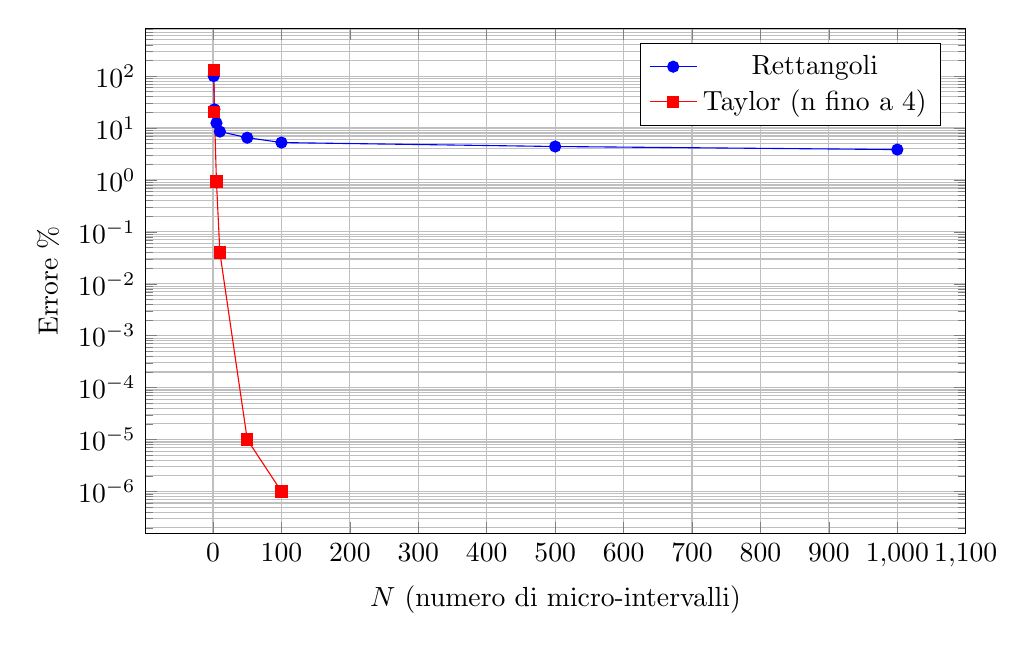
\begin{tikzpicture}
\begin{axis}[
    width=12cm,
    height=8cm,
    xlabel={$N$ (numero di micro-intervalli)},
    ylabel={Errore \%},
    ymode=log,
    grid=both,
    legend pos=north east
]

% Dati rettangoli
\addplot[
    color=blue,
    mark=*,
] coordinates {
    (1,100)
    (2,22.85)
    (5,12.43)
    (10,8.53)
    (50,6.50)
    (100,5.24)
    (500,4.40)
    (1000,3.84)
};
\addlegendentry{Rettangoli}

% Dati Taylor (n fino a 4)
\addplot[
    color=red,
    mark=square*,
] coordinates {
    (1,128.82)
    (2,19.98)
    (5,0.93)
    (10,0.04)
    (50,0.00001)
    (100,0.000001)
    (500,0.0)
    (1000,0.0)
};
\addlegendentry{Taylor (n fino a 4)}

\end{axis}
\end{tikzpicture}
\caption{Confronto dell'errore percentuale tra la regola dei rettangoli e il metodo dei micro-integrali basato sulla serie di Taylor.}
\end{figure}
\section{Conclusioni}

Abbiamo confrontato tre metodi per calcolare l'integrale definito
\(\int_0^1 x^3 e^{x^2} \, dx \approx 0.5\):

\begin{itemize}
    \item \textbf{Integrale classico}: calcolato con metodi analitici o software simbolico.
    \item \textbf{Somma di Riemann / regola dei rettangoli}: suddivisione dell'intervallo in \(N\) micro-intervalli e somma dei valori della funzione all'inizio di ciascun intervallo:
    \[
    \int_a^b f(x) \, dx \approx \sum_{k=0}^{N-1} f(x_k) \Delta, \quad x_k = a + k \Delta, \quad \Delta = \frac{b-a}{N}.
    \]
    \item \textbf{Micro-integrali con espansione di Taylor}: somma dei micro-intervalli usando la serie di Taylor centrata nel punto medio di ciascun intervallo:
    \[
    \int_a^b f(x) \, dx \approx \sum_{k=0}^{N-1} \sum_{\substack{n=0 \\ n \text{ pari}}}^{n_\text{max}} 
    \frac{f^{(n)}(c_k)}{(n+1)!} \Delta^{\,n+1} 2^{-n}, \quad 
    c_k = x_k + \frac{\Delta}{2}.
    \]
\end{itemize}

Dal confronto emerge che già con pochi micro-intervalli e pochi termini pari della serie di Taylor si ottiene un'approssimazione molto vicina al valore reale, mentre la semplice somma di Riemann richiede molti più intervalli per raggiungere la stessa precisione.  

Questo dimostra che l'uso della serie di Taylor su micro-intervalli può migliorare significativamente la convergenza della somma, specialmente per funzioni complesse o rapidamente varianti.

\end{document}